% Options for packages loaded elsewhere
\PassOptionsToPackage{unicode}{hyperref}
\PassOptionsToPackage{hyphens}{url}
\documentclass[
]{ltjsarticle}
\usepackage{xcolor}
\usepackage{amsmath,amssymb}
\setcounter{secnumdepth}{-\maxdimen} % remove section numbering
\usepackage{iftex}
\ifPDFTeX
  \usepackage[T1]{fontenc}
  \usepackage[utf8]{inputenc}
  \usepackage{textcomp} % provide euro and other symbols
\else % if luatex or xetex
  \usepackage{unicode-math} % this also loads fontspec
  \defaultfontfeatures{Scale=MatchLowercase}
  \defaultfontfeatures[\rmfamily]{Ligatures=TeX,Scale=1}
\fi
\usepackage{lmodern}
\ifPDFTeX\else
  % xetex/luatex font selection
\fi
% Use upquote if available, for straight quotes in verbatim environments
\IfFileExists{upquote.sty}{\usepackage{upquote}}{}
\IfFileExists{microtype.sty}{% use microtype if available
  \usepackage[]{microtype}
  \UseMicrotypeSet[protrusion]{basicmath} % disable protrusion for tt fonts
}{}
\makeatletter
\@ifundefined{KOMAClassName}{% if non-KOMA class
  \IfFileExists{parskip.sty}{%
    \usepackage{parskip}
  }{% else
    \setlength{\parindent}{0pt}
    \setlength{\parskip}{6pt plus 2pt minus 1pt}}
}{% if KOMA class
  \KOMAoptions{parskip=half}}
\makeatother
\usepackage{longtable,booktabs,array}
\newcounter{none} % for unnumbered tables
\usepackage{calc} % for calculating minipage widths
% Correct order of tables after \paragraph or \subparagraph
\usepackage{etoolbox}
\makeatletter
\patchcmd\longtable{\par}{\if@noskipsec\mbox{}\fi\par}{}{}
\makeatother
% Allow footnotes in longtable head/foot
\IfFileExists{footnotehyper.sty}{\usepackage{footnotehyper}}{\usepackage{footnote}}
\makesavenoteenv{longtable}
\usepackage{graphicx}
\makeatletter
\newsavebox\pandoc@box
\newcommand*\pandocbounded[1]{% scales image to fit in text height/width
  \sbox\pandoc@box{#1}%
  \Gscale@div\@tempa{\textheight}{\dimexpr\ht\pandoc@box+\dp\pandoc@box\relax}%
  \Gscale@div\@tempb{\linewidth}{\wd\pandoc@box}%
  \ifdim\@tempb\p@<\@tempa\p@\let\@tempa\@tempb\fi% select the smaller of both
  \ifdim\@tempa\p@<\p@\scalebox{\@tempa}{\usebox\pandoc@box}%
  \else\usebox{\pandoc@box}%
  \fi%
}
% Set default figure placement to htbp
\def\fps@figure{htbp}
\makeatother
\setlength{\emergencystretch}{3em} % prevent overfull lines
\providecommand{\tightlist}{%
  \setlength{\itemsep}{0pt}\setlength{\parskip}{0pt}}
\usepackage{bookmark}
\IfFileExists{xurl.sty}{\usepackage{xurl}}{} % add URL line breaks if available
\urlstyle{same}
\hypersetup{
  pdftitle={球面投影 (radial projection) の定義と中心投影との関係},
  pdfauthor={木原 範昭（Noriaki Kihara）},
  hidelinks,
  pdfcreator={LaTeX via pandoc}}

\title{球面投影 (radial projection) の定義と中心投影との関係}
\usepackage{etoolbox}
\makeatletter
\providecommand{\subtitle}[1]{% add subtitle to \maketitle
  \apptocmd{\@title}{\par {\large #1 \par}}{}{}
}
\makeatother
\subtitle{中心投影フレームワークの基礎写像としての位置付け（テクニカルノート）}
\author{木原 範昭（Noriaki Kihara）}
\date{2026-05}

\begin{document}
\maketitle

\textbf{Concept
DOI（最新版に自動転送）}：\href{https://doi.org/10.5281/zenodo.20462569}{10.5281/zenodo.20462569}
\textbf{v3.2 Version
DOI}：\href{https://doi.org/10.5281/zenodo.20500187}{10.5281/zenodo.20500187}
\textbf{Zenodo ページ}：\url{https://zenodo.org/records/20500187}

\section{本ノートの性格}\label{ux672cux30ceux30fcux30c8ux306eux6027ux683c}

\textbf{本稿は中心投影フレームワーク {[}1{]}, {[}2{]}
の基礎写像を明示的に定義・整理するテクニカルノートである。}

本ノートが扱う写像

\[\sigma_R: \mathbb{R}^{n+1} \setminus \{0\} \to S^n(R), \quad \sigma_R(x) = \frac{R}{\|x\|} \cdot x\]

は、位相幾何学において \textbf{radial
projection（動径射影）}、線形代数・微分幾何において \textbf{正規化写像
(normalization map)}、変形レトラクトの典型例（{[}Hatcher,
Ch.0{]}）として古典的に既知である。本ノートは新規の幾何学的定理を主張せず、以下のみを行う：

\begin{itemize}
\tightlist
\item
  この写像を \textbf{「球面投影 \(\sigma_R\)」}
  と呼称し、記号を固定する（§2）
\item
  著者の中心投影 {[}1{]} および合成演算 {[}2{]} が、球面投影の接超平面
  \(\Pi_R\) への制限として特徴付けられることを示す（§3）
\item
  \(\sigma_R\) と中心投影 \(\Phi_R\)
  の単射性・像・微分構造の対比を整理する（§3）
\end{itemize}

ジャーナル投稿ではなく、著者の中心投影シリーズの\textbf{基礎を固める
Zenodo プレプリント}として公開する。

\begin{center}\rule{0.5\linewidth}{0.5pt}\end{center}

\section{§1 序論}\label{ux5e8fux8ad6}

\subsection{1.1 動機}\label{ux52d5ux6a5f}

ベクトルを正規化して指定半径の球面に写す写像 \(x \mapsto (R/\|x\|) x\)
は、位相幾何学において \textbf{radial projection} または
\textbf{動径レトラクト}として、線形代数において \textbf{正規化写像
(normalization map)} として古典的に既知である。例えば Hatcher
『Algebraic Topology』Chapter 0 では、\(\mathbb{R}^n \setminus \{0\}\)
から \(S^{n-1}\)
への変形レトラクトの典型例として登場し、ホモトピー同値の最も基本的な例として扱われる。

本ノートでは、この既知の写像に著者の中心投影フレームワーク {[}1{]},
{[}2{]} 内で用いる記号 \(\sigma_R\)
を固定し、必要な基本性質を一箇所に整理する。多くの教科書ではこの写像が中間計算または例として扱われるため、シリーズ内での参照基盤として明示的なノートが有用と判断した。

本ノートはこの基礎的写像を「球面投影
\(\sigma_R\)」と呼称して記号を固定し、著者の中心投影フレームワーク
{[}1{]}, {[}2{]} における操作との関係を明示することを目的とする。

\subsection{1.2
既存中心投影フレームワークとの関係}\label{ux65e2ux5b58ux4e2dux5fc3ux6295ux5f71ux30d5ux30ecux30fcux30e0ux30efux30fcux30afux3068ux306eux95a2ux4fc2}

著者は先行論文 {[}1{]} において、中心投影 \(\Phi_R: \Pi_R \to S^n(R)\)
による 4 次元時空の幾何学的定式化を与えた。さらに {[}2{]}
において、複数軸での次元削減操作が「複数回の中心投影」ではなく「\textbf{1
回の中心投影と球面上の可換切断}」として正しく代数化されることを示した。

本ノートは、これら既存の中心投影が、より広い定義域を持つ球面投影
\(\sigma_R\) の\textbf{接超平面 \(\Pi_R\)
への制限}として特徴付けられることを示す（補題 3.2）。

なお、{[}1{]} における「中心投影」\(\Phi_R: \Pi_R \to S^n(R)\)
は、古典地図学における gnomonic
projection（心射図法、\(S^n_+ \to \Pi_R\)）と\textbf{向きが逆}である。本ノートおよび
{[}1{]} では、接超平面を始域、球面を終域とする向きを採る。

\subsection{1.3
本ノートの射程}\label{ux672cux30ceux30fcux30c8ux306eux5c04ux7a0b}

本ノートは以下のみを扱う：

\begin{itemize}
\tightlist
\item
  球面投影 \(\sigma_R\) の定義と基本性質
\item
  中心投影 \(\Phi_R\) との関係（特殊化としての位置付け）
\item
  \(\Phi_R\) の像と単射性、\(\sigma_R\) の非単射性の対比
\end{itemize}

以下は本ノートの射程外である：

\begin{itemize}
\tightlist
\item
  球面投影の物理的解釈・応用（曲率、時空、量子論等）
\item
  {[}1{]}, {[}2{]} の具体的応用（誘導計量、Einstein
  テンソル、ブラックホール熱力学等）
\item
  等径関数・極作用といった抽象的部分多様体論との対応
\item
  ステレオ射影（共形）など他の球面関連写像との比較
\end{itemize}

これらは別ノートまたは別論文において扱う。

\subsection{1.4
用語に関する注意}\label{ux7528ux8a9eux306bux95a2ux3059ux308bux6ce8ux610f}

「球面投影 (spherical
projection)」という語は文献によって異なる意味で用いられる（ステレオ射影、各種地図投影など）。本ノートでは
\(\sigma_R\) をこの名で呼ぶが、これは位相幾何学の標準術語 \textbf{radial
projection} と同じ写像である。読者の混乱を避けるため、本文では括弧書きで
radial projection を併記する。

\begin{center}\rule{0.5\linewidth}{0.5pt}\end{center}

\section{§2
球面投影の定義と基本性質}\label{ux7403ux9762ux6295ux5f71ux306eux5b9aux7fa9ux3068ux57faux672cux6027ux8cea}

\subsection{2.1 定義}\label{ux5b9aux7fa9}

\textbf{定義 2.1（球面投影 / radial projection）}：正の実数 \(R > 0\)
に対し、球面投影 \(\sigma_R\) を以下で定める：

\[\sigma_R: \mathbb{R}^{n+1} \setminus \{0\} \to S^n(R), \quad \sigma_R(x) = \frac{R}{\|x\|} \cdot x \tag{2.1}\]

ここで \(S^n(R) = \{y \in \mathbb{R}^{n+1} \mid \|y\| = R\}\) は半径
\(R\) の \(n\) 次元球面、\(\|\cdot\|\) は標準ユークリッドノルム。

\textbf{Well-definedness}：\(\|\sigma_R(x)\| = (R/\|x\|) \cdot \|x\| = R\)
より \(\sigma_R(x) \in S^n(R)\)。

\subsection{2.2 基本性質}\label{ux57faux672cux6027ux8cea}

\textbf{命題 2.1（基本性質）}：

\begin{enumerate}
\def\labelenumi{(\roman{enumi})}
\item
  \(\sigma_R\) は \(\mathbb{R}^{n+1} \setminus \{0\}\) 全域で
  \(C^\infty\) 級である（部分多様体 \(S^n(R) \subset \mathbb{R}^{n+1}\)
  への滑らかな写像）。
\item
  \(\sigma_R\) は \textbf{\(S^n(R)\)
  上へのレトラクション}である：\(\sigma_R \big|_{S^n(R)} = \mathrm{id}_{S^n(R)}\)。特に全射。
\item
  任意の \(t > 0\) と \(x \in \mathbb{R}^{n+1} \setminus \{0\}\) に対し
  \(\sigma_R(tx) = \sigma_R(x)\)。
\end{enumerate}

\textbf{証明}：

\begin{enumerate}
\def\labelenumi{(\roman{enumi})}
\item
  \(\|x\| > 0\) なので \(1/\|x\|\) は \(C^\infty\)、線形写像
  \(x \mapsto x\) も \(C^\infty\)、これらの積は \(C^\infty\)。
\item
  \(y \in S^n(R)\) なら
  \(\|y\| = R\)、\(\sigma_R(y) = (R/R) y = y\)。よって
  \(S^n(R) \subset \mathrm{Im}(\sigma_R)\)、すなわち全射。
\item
  \(\sigma_R(tx) = (R/\|tx\|)(tx) = (R/(t\|x\|))(tx) = (R/\|x\|) x = \sigma_R(x)\)。\(\square\)
\end{enumerate}

\textbf{脚注（\(t < 0\) の扱い）}：\(t < 0\) の場合は
\(\sigma_R(tx) = -\sigma_R(x)\) となり、向きが反転する。性質 (iii)
が同一視するのは原点を通る\textbf{正の半直線} \(\{tx : t > 0\}\)
であり、両側の直線ではない。

\subsection{2.3
冪等性とレトラクト構造}\label{ux51aaux7b49ux6027ux3068ux30ecux30c8ux30e9ux30afux30c8ux69cbux9020}

\textbf{命題 2.2（冪等性）}：\(\sigma_R\) を
\(\mathbb{R}^{n+1} \setminus \{0\}\) の自己写像とみなせば
\(\sigma_R \circ \sigma_R = \sigma_R\)。

\textbf{証明}：\(\sigma_R(x) \in S^n(R)\) なので、命題 2.1(ii) より
\(\sigma_R(\sigma_R(x)) = \sigma_R(x)\)。\(\square\)

これは「projection」という語を正当化する：\(\sigma_R\) は像 \(S^n(R)\)
への射影演算子である。

\textbf{変形レトラクト}：ホモトピー
\(H(x, s) = (1-s) x + s \cdot \sigma_R(x)\)（\(s \in [0, 1]\)）は
\(\mathbb{R}^{n+1} \setminus \{0\}\) の \(S^n(R)\)
への\textbf{強変形レトラクト}を与える（古典的、{[}Hatcher Ch.0{]}
参照）。

\subsection{2.4
商空間としての特徴}\label{ux5546ux7a7aux9593ux3068ux3057ux3066ux306eux7279ux5fb4}

正の実数群 \(\mathbb{R}_{>0}\) がスカラー乗法 \(t \cdot x = tx\) により
\(\mathbb{R}^{n+1} \setminus \{0\}\) に作用する。

\textbf{命題 2.3（商空間）}：商空間

\[(\mathbb{R}^{n+1} \setminus \{0\}) / \mathbb{R}_{>0} \cong S^n(R)\]

であり、\(\sigma_R\) は各正の半直線（軌道）から半径 \(R\)
の代表点を選ぶ標準切断と解釈される。

\textbf{証明}：商写像
\(\pi: \mathbb{R}^{n+1} \setminus \{0\} \to (\mathbb{R}^{n+1} \setminus \{0\}) / \mathbb{R}_{>0}\)
と \(\sigma_R\) は同じファイバー \(\{tx : t > 0\}\) を持つので、写像
\(\overline{\sigma_R}: (\mathbb{R}^{n+1} \setminus \{0\}) / \mathbb{R}_{>0} \to S^n(R)\)
が誘導され、これは全単射。連続性・可微性は標準的。\(\square\)

これは命題 2.1(iii)
の構造的な言い換えで、\textbf{動径方向の情報が完全に捨てられる}ことを商構造として明示する。

\subsection{2.5 微分構造}\label{ux5faeux5206ux69cbux9020}

\textbf{命題 2.4（微分の核と像）}：各
\(x \in \mathbb{R}^{n+1} \setminus \{0\}\) における \(\sigma_R\) の微分
\(D\sigma_R|_x: \mathbb{R}^{n+1} \to T_{\sigma_R(x)} S^n(R)\) は

\[D\sigma_R|_x (v) = \frac{R}{\|x\|}\left(v - \frac{x \cdot v}{\|x\|^2} x\right) \tag{2.2}\]

であり、その核は

\[\ker D\sigma_R|_x = \mathrm{span}\{x\} \tag{2.3}\]

すなわち \(x\) 方向（動径方向）。\(D\sigma_R|_x\) は階数 \(n\)
の沈め込みであり、その像は

\[\mathrm{Im}(D\sigma_R|_x) = x^\perp = T_{\sigma_R(x)} S^n(R) \tag{2.4}\]

である（\(\sigma_R(x)\) は \(x\) の正のスカラー倍なので、\(\sigma_R(x)\)
における球面 \(S^n(R)\) の接空間は \(x\) の直交補空間 \(x^\perp\)
に等しい）。

\textbf{証明}：\(\|x\|^{-1}\) の方向 \(v\) に沿った微分が
\(-\|x\|^{-3}(x \cdot v)\)
であることを用いて、\(\sigma_R(x) = R \|x\|^{-1} x\) を方向 \(v\)
に微分すると

\[D\sigma_R|_x(v) = R \big(-\|x\|^{-3} (x \cdot v)\big) x + R \|x\|^{-1} v = -R \|x\|^{-3} (x \cdot v) x + R \|x\|^{-1} v\]

これを整理すると (2.2)。核について、\(D\sigma_R|_x(v) = 0\) とすると

\[v - \frac{x \cdot v}{\|x\|^2} x = 0\]

である。したがって

\[v = \frac{x \cdot v}{\|x\|^2} x\]

となり、\(v\) は \(x\) のスカラー倍である。逆に \(v = \lambda x\)
とおけば

\[v - \frac{x \cdot v}{\|x\|^2} x = \lambda x - \frac{\lambda \|x\|^2}{\|x\|^2} x = 0\]

なので \(D\sigma_R|_x(v) = 0\)。ゆえに
\(\ker D\sigma_R|_x = \mathrm{span}\{x\}\)。

像について、任意の \(v\) に対し
\(x \cdot D\sigma_R|_x(v) = \frac{R}{\|x\|}\left(x \cdot v - \frac{x \cdot v}{\|x\|^2}\|x\|^2\right) = 0\)
であるから
\(\mathrm{Im}(D\sigma_R|_x) \subseteq x^\perp\)。階数・退化次数定理より
\(\dim \mathrm{Im}(D\sigma_R|_x) = (n+1) - \dim \ker D\sigma_R|_x = n = \dim x^\perp\)
なので、\(\mathrm{Im}(D\sigma_R|_x) = x^\perp = T_{\sigma_R(x)} S^n(R)\)。\(\square\)

これにより、\textbf{動径方向は微分の核に正確に対応し、接方向のみが球面に写る}という球面投影の微分幾何学的構造が明確化される。

\subsection{2.6
角度成分の保存}\label{ux89d2ux5ea6ux6210ux5206ux306eux4fddux5b58}

\textbf{命題 2.5（角度の保存）}：任意の
\(x, y \in \mathbb{R}^{n+1} \setminus \{0\}\) に対し

\[\angle(\sigma_R(x), \sigma_R(y)) = \angle(x, y) \tag{2.5}\]

ここで \(\angle(\cdot, \cdot)\) はベクトル間の非有向角度。

\textbf{証明}：

\[\frac{\sigma_R(x) \cdot \sigma_R(y)}{\|\sigma_R(x)\| \cdot \|\sigma_R(y)\|} = \frac{(R/\|x\|)(R/\|y\|)(x \cdot y)}{R \cdot R} = \frac{x \cdot y}{\|x\| \cdot \|y\|}\]

すなわち余弦値が一致し、角度は等しい。\(\square\)

\textbf{注意（用語）}：本性質は二つのベクトル間の角度の保存であり、共形写像（曲線間の角度を保存する写像）とは異なる概念である。\(\sigma_R\)
は次元を落とすため、曲線間の角度の保存性は意味を成さない。

\subsection{2.7
スケール不変性}\label{ux30b9ux30b1ux30fcux30ebux4e0dux5909ux6027}

\textbf{命題 2.6（半径スケールに対する方向の不変性）}：任意の
\(R_1, R_2 > 0\) と \(x \in \mathbb{R}^{n+1} \setminus \{0\}\)
に対し、\(\sigma_{R_1}(x)\) と \(\sigma_{R_2}(x)\) は原点 \(O\) から
\(x\) への正の半直線上にある。

\textbf{証明}：\(\sigma_{R_1}(x) = (R_1/\|x\|) x\),
\(\sigma_{R_2}(x) = (R_2/\|x\|) x\) はいずれも \(x\)
の正のスカラー倍。\(\square\)

すなわち、球面投影において\textbf{方向成分は半径 \(R\)
のスケールに対し不変}である。

\begin{figure}
\centering
\pandocbounded{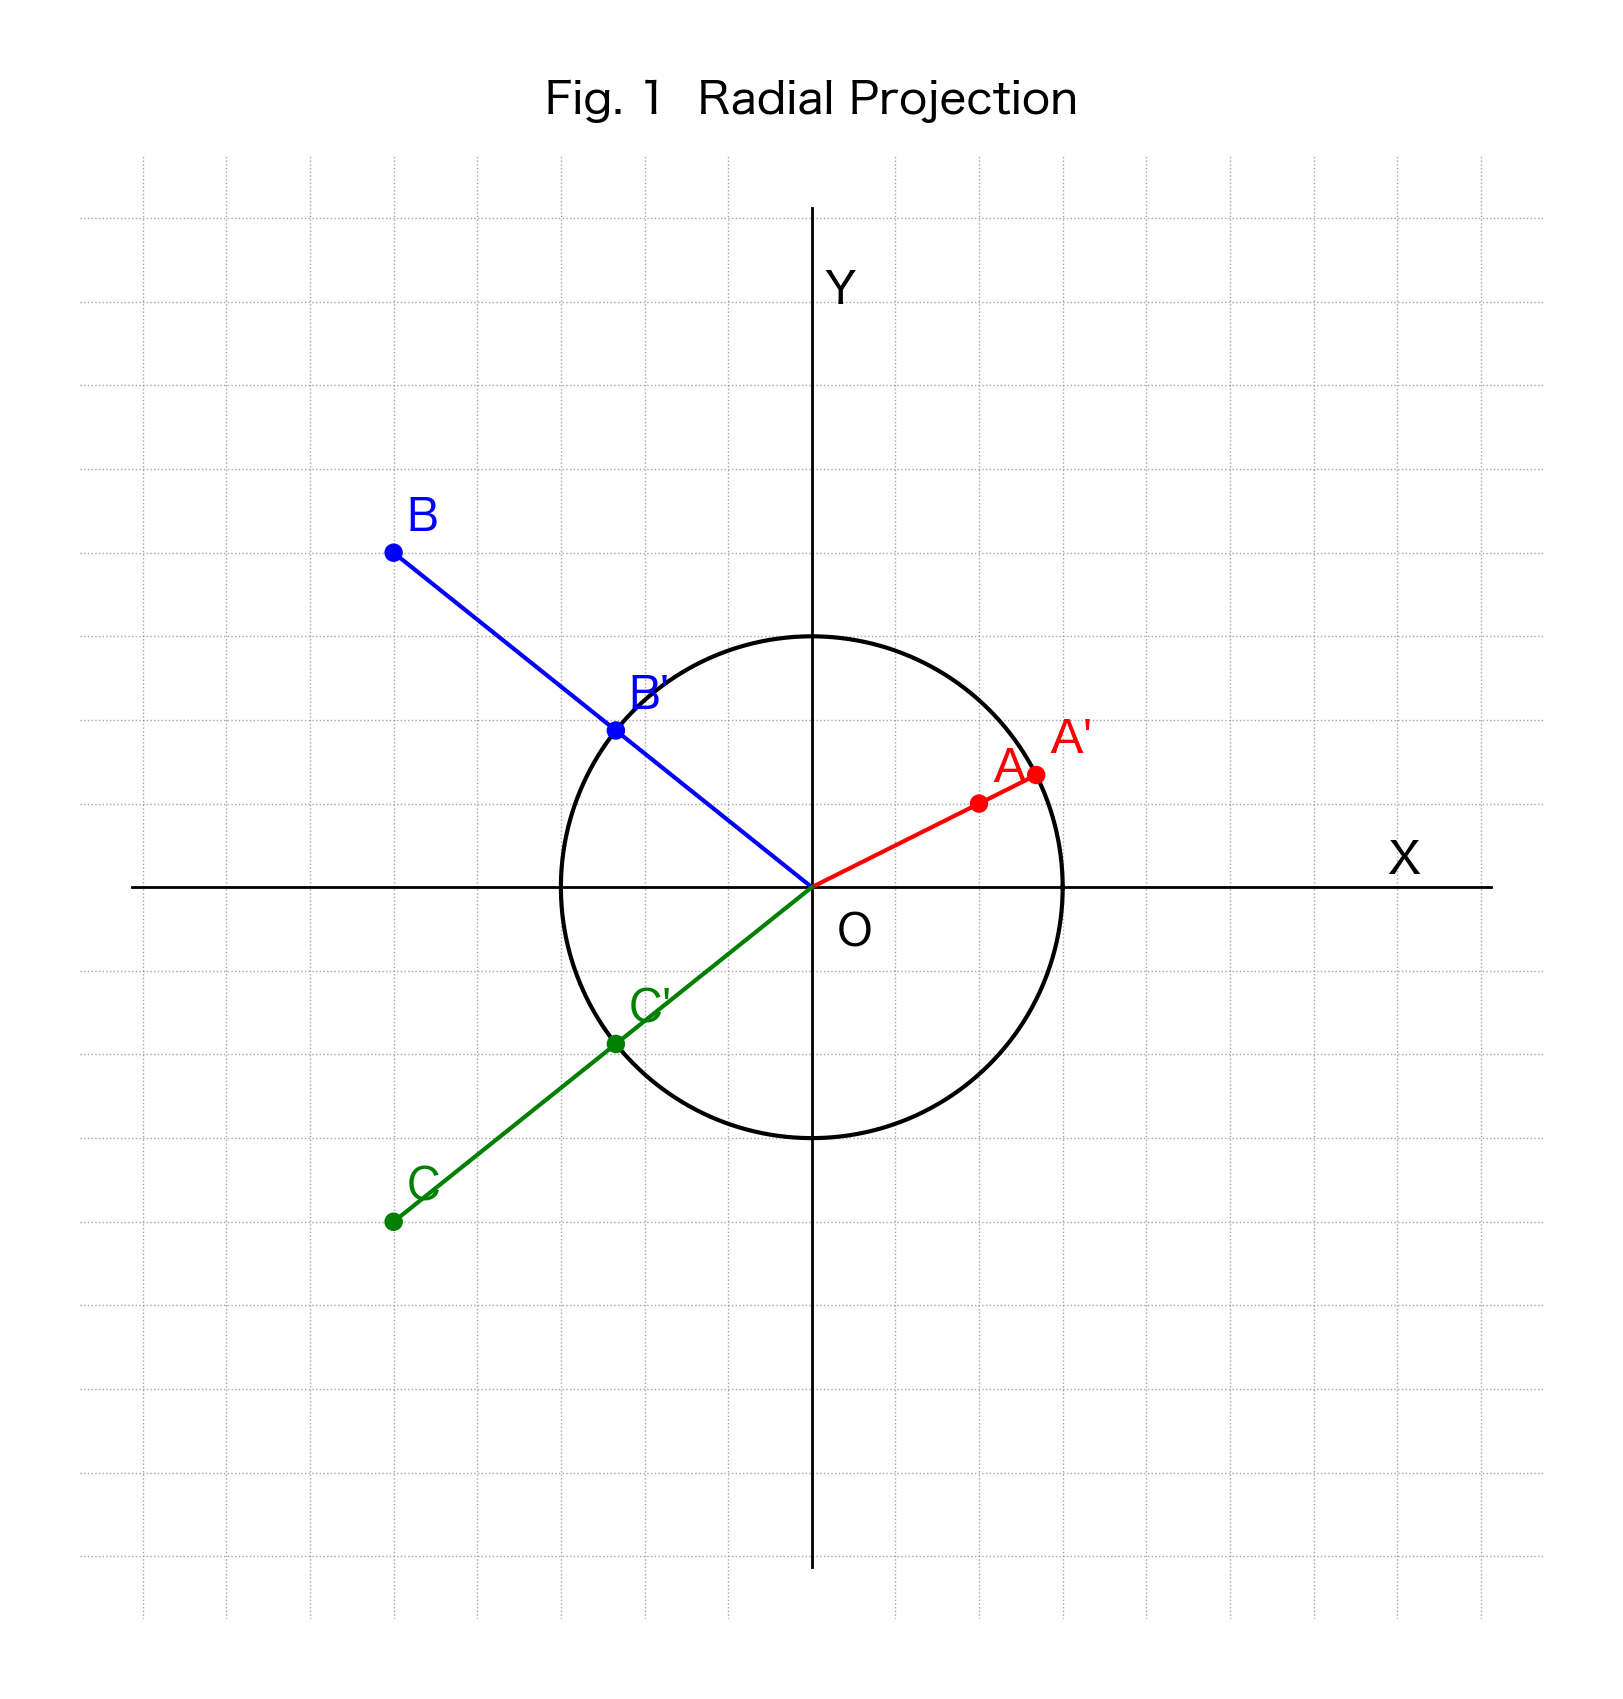
\includegraphics[keepaspectratio,alt={Fig. 1 Radial Projection}]{fig1_radial_projection.png}}
\caption{Fig. 1 Radial Projection}
\end{figure}

\textbf{図 1}：球面投影 \(\sigma_R\) の図解（\(n=1\)、\(R=3\)）。原点
\(O\) を視点とする放射状半直線上で、点
\(A\)（円の内側）、\(B, C\)（円の外側、異なる象限）はそれぞれ円周上の
\(A', B', C'\) に投影される。

\begin{figure}
\centering
\pandocbounded{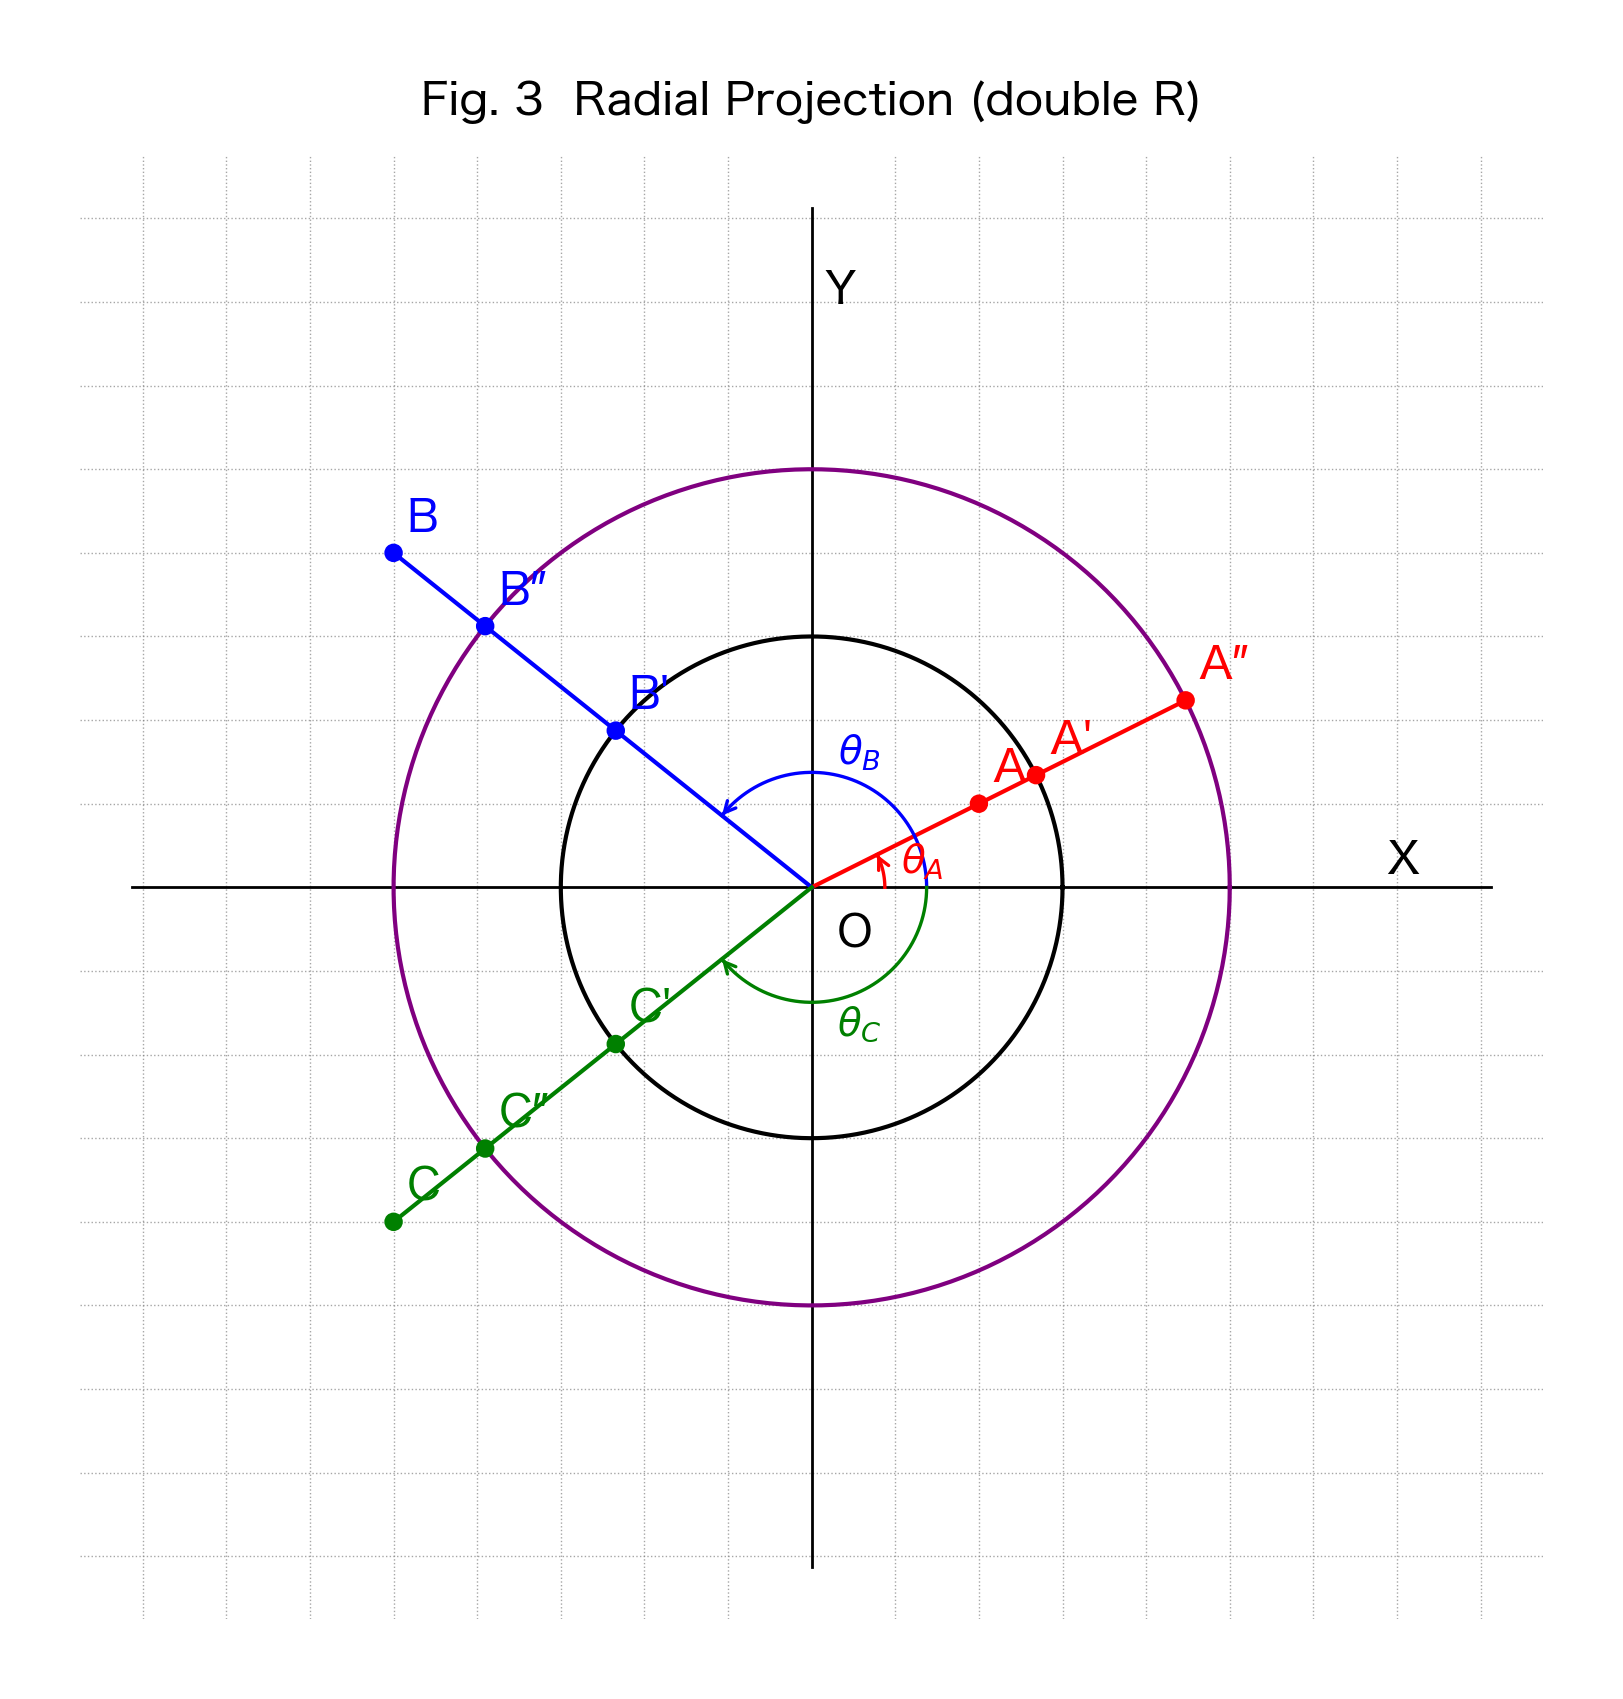
\includegraphics[keepaspectratio,alt={Fig. 3 Radial Projection (double R)}]{fig3_radial_projection_double_R.png}}
\caption{Fig. 3 Radial Projection (double R)}
\end{figure}

\textbf{図 3}：球面投影における半径スケールに対する方向不変性（命題
2.6）。半径 \(R=3\)（黒円）と \(R=5\)（紫円）の双方に対し、点
\(A, B, C\) の像は同一の放射状半直線上に並ぶ。したがって、各点と \(x\)
軸正方向のなす角 \(\theta_A, \theta_B, \theta_C\) は \(R\)
に依らず保存される。

\begin{center}\rule{0.5\linewidth}{0.5pt}\end{center}

\section{§3
中心投影との関係}\label{ux4e2dux5fc3ux6295ux5f71ux3068ux306eux95a2ux4fc2}

\subsection{3.1
中心投影の定義}\label{ux4e2dux5fc3ux6295ux5f71ux306eux5b9aux7fa9}

\textbf{定義 3.1（中心投影）}：球面 \(S^n(R)\) の北極
\(N = (0, \ldots, 0, R)\) における接超平面を

\[\Pi_R = \{x \in \mathbb{R}^{n+1} \mid x_{n+1} = R\} \tag{3.1}\]

と定める。\(\Pi_R \cong \mathbb{R}^n\)。中心投影 \(\Phi_R\)
を以下で定める：

\[\Phi_R: \Pi_R \to S^n_+(R), \quad \Phi_R(x) = \frac{R}{\|x\|} \cdot x \tag{3.2}\]

ここで \(S^n_+(R) = \{y \in S^n(R) \mid y_{n+1} > 0\}\)
は\textbf{開上半球面}である。これが \(\Phi_R\) の像であることは下記命題
3.1 で示す。

これは {[}1{]} §2
で定義された中心投影と一致する（最終座標の正値性については {[}1{]} 注釈
3.1 参照）。

\textbf{注釈（向きについて）}：本定義の \(\Phi_R\)
は\textbf{接超平面を始域、球面を終域}とする向きである。古典地図学における
gnomonic projection（心射図法）は逆向き（球面 →
接平面）で定義されることが多いので、用語上の混同に注意。

\subsection{3.2
中心投影の像と単射性}\label{ux4e2dux5fc3ux6295ux5f71ux306eux50cfux3068ux5358ux5c04ux6027}

\textbf{命題 3.1（\(\Phi_R\) の像と単射性）}：

\begin{enumerate}
\def\labelenumi{(\roman{enumi})}
\item
  \(\Phi_R\) の像は開上半球面
  \(S^n_+(R) = \{y \in S^n(R) \mid y_{n+1} > 0\}\) である。
\item
  \(\Phi_R: \Pi_R \to S^n_+(R)\) は
  \textbf{微分同相}である（特に単射）。
\end{enumerate}

\textbf{証明}：

\begin{enumerate}
\def\labelenumi{(\roman{enumi})}
\item
  \(x \in \Pi_R\) は \(x_{n+1} = R\) なので、\(\Phi_R(x)\) の最終座標は
  \((R/\|x\|) \cdot R = R^2/\|x\| > 0\)。よって
  \(\Phi_R(\Pi_R) \subset S^n_+(R)\)。逆に任意の \(y \in S^n_+(R)\)
  に対し \(y_{n+1} > 0\)、\(x := (R/y_{n+1}) y\) とおけば
  \(x_{n+1} = R\) なので
  \(x \in \Pi_R\)、\(\|x\| = R\|y\|/y_{n+1} = R^2/y_{n+1}\)、\(\Phi_R(x) = (R/\|x\|) x = (y_{n+1}/R) \cdot (R/y_{n+1}) y = y\)。よって全射。
\item
  \begin{enumerate}
  \def\labelenumii{(\roman{enumii})}
  \tightlist
  \item
    の構成は逆写像 \(\Phi_R^{-1}(y) = (R/y_{n+1}) y\) を与え、両方向で
    \(C^\infty\)。\(\square\)
  \end{enumerate}
\end{enumerate}

\subsection{3.3
球面投影と中心投影の関係}\label{ux7403ux9762ux6295ux5f71ux3068ux4e2dux5fc3ux6295ux5f71ux306eux95a2ux4fc2}

\textbf{補題 3.2（中心投影は球面投影の制限）}：中心投影 \(\Phi_R\)
は、球面投影 \(\sigma_R\) の定義域を \(\Pi_R\) に制限したものと、像を
\(S^n_+(R)\) に制限したものに一致する：

\[\Phi_R = \sigma_R \big|_{\Pi_R}: \Pi_R \to S^n_+(R) \tag{3.3}\]

\textbf{証明}：定義 2.1 の写像式 \(\sigma_R(x) = (R/\|x\|) x\) と定義
3.1 の写像式 \(\Phi_R(x) = (R/\|x\|) x\)
は完全に同一。\(\Pi_R \subset \mathbb{R}^{n+1} \setminus \{0\}\)（\(\Pi_R\)
上 \(x_{n+1} = R > 0\) なので原点でない）であり、\(\sigma_R\) の定義域を
\(\Pi_R\) に制限すれば \(\Phi_R\) と一致する。像が \(S^n_+(R)\)
に収まることは命題 3.1(i) より。\(\square\)

\subsection{\texorpdfstring{3.4 \(\sigma_R\) と \(\Phi_R\)
の対比}{3.4 \textbackslash sigma\_R と \textbackslash Phi\_R の対比}}\label{sigma_r-ux3068-phi_r-ux306eux5bfeux6bd4}

{\def\LTcaptype{none} % do not increment counter
\begin{longtable}[]{@{}
  >{\raggedright\arraybackslash}p{(\linewidth - 4\tabcolsep) * \real{0.3333}}
  >{\raggedright\arraybackslash}p{(\linewidth - 4\tabcolsep) * \real{0.3333}}
  >{\raggedright\arraybackslash}p{(\linewidth - 4\tabcolsep) * \real{0.3333}}@{}}
\toprule\noalign{}
\begin{minipage}[b]{\linewidth}\raggedright
性質
\end{minipage} & \begin{minipage}[b]{\linewidth}\raggedright
\(\sigma_R\)
\end{minipage} & \begin{minipage}[b]{\linewidth}\raggedright
\(\Phi_R\)
\end{minipage} \\
\midrule\noalign{}
\endhead
\bottomrule\noalign{}
\endlastfoot
定義域 & \(\mathbb{R}^{n+1} \setminus \{0\}\) &
\(\Pi_R\)（接超平面、\(\mathbb{R}^n\) と同型） \\
像 & \(S^n(R)\)（全球面） & \(S^n_+(R)\)（\textbf{開上半球面のみ}） \\
単射性 & \textbf{非単射}（半直線を 1 点に潰す） &
\textbf{単射}（微分同相） \\
動径方向 & 核に含まれる（命題 2.4） &
核の方向が定義域の接空間に含まれない（横断的） \\
\end{longtable}
}

この対比は本ノートの\textbf{核心}である。球面投影は定義域を
\(\mathbb{R}^{n+1} \setminus \{0\}\)
全体に拡張する代償として単射性を失う。一方、中心投影は単射性と豊かな幾何構造（誘導計量、曲率等）を保つが、定義域は
\(\Pi_R\)、像は \(S^n_+(R)\) に限定される。

\begin{figure}
\centering
\pandocbounded{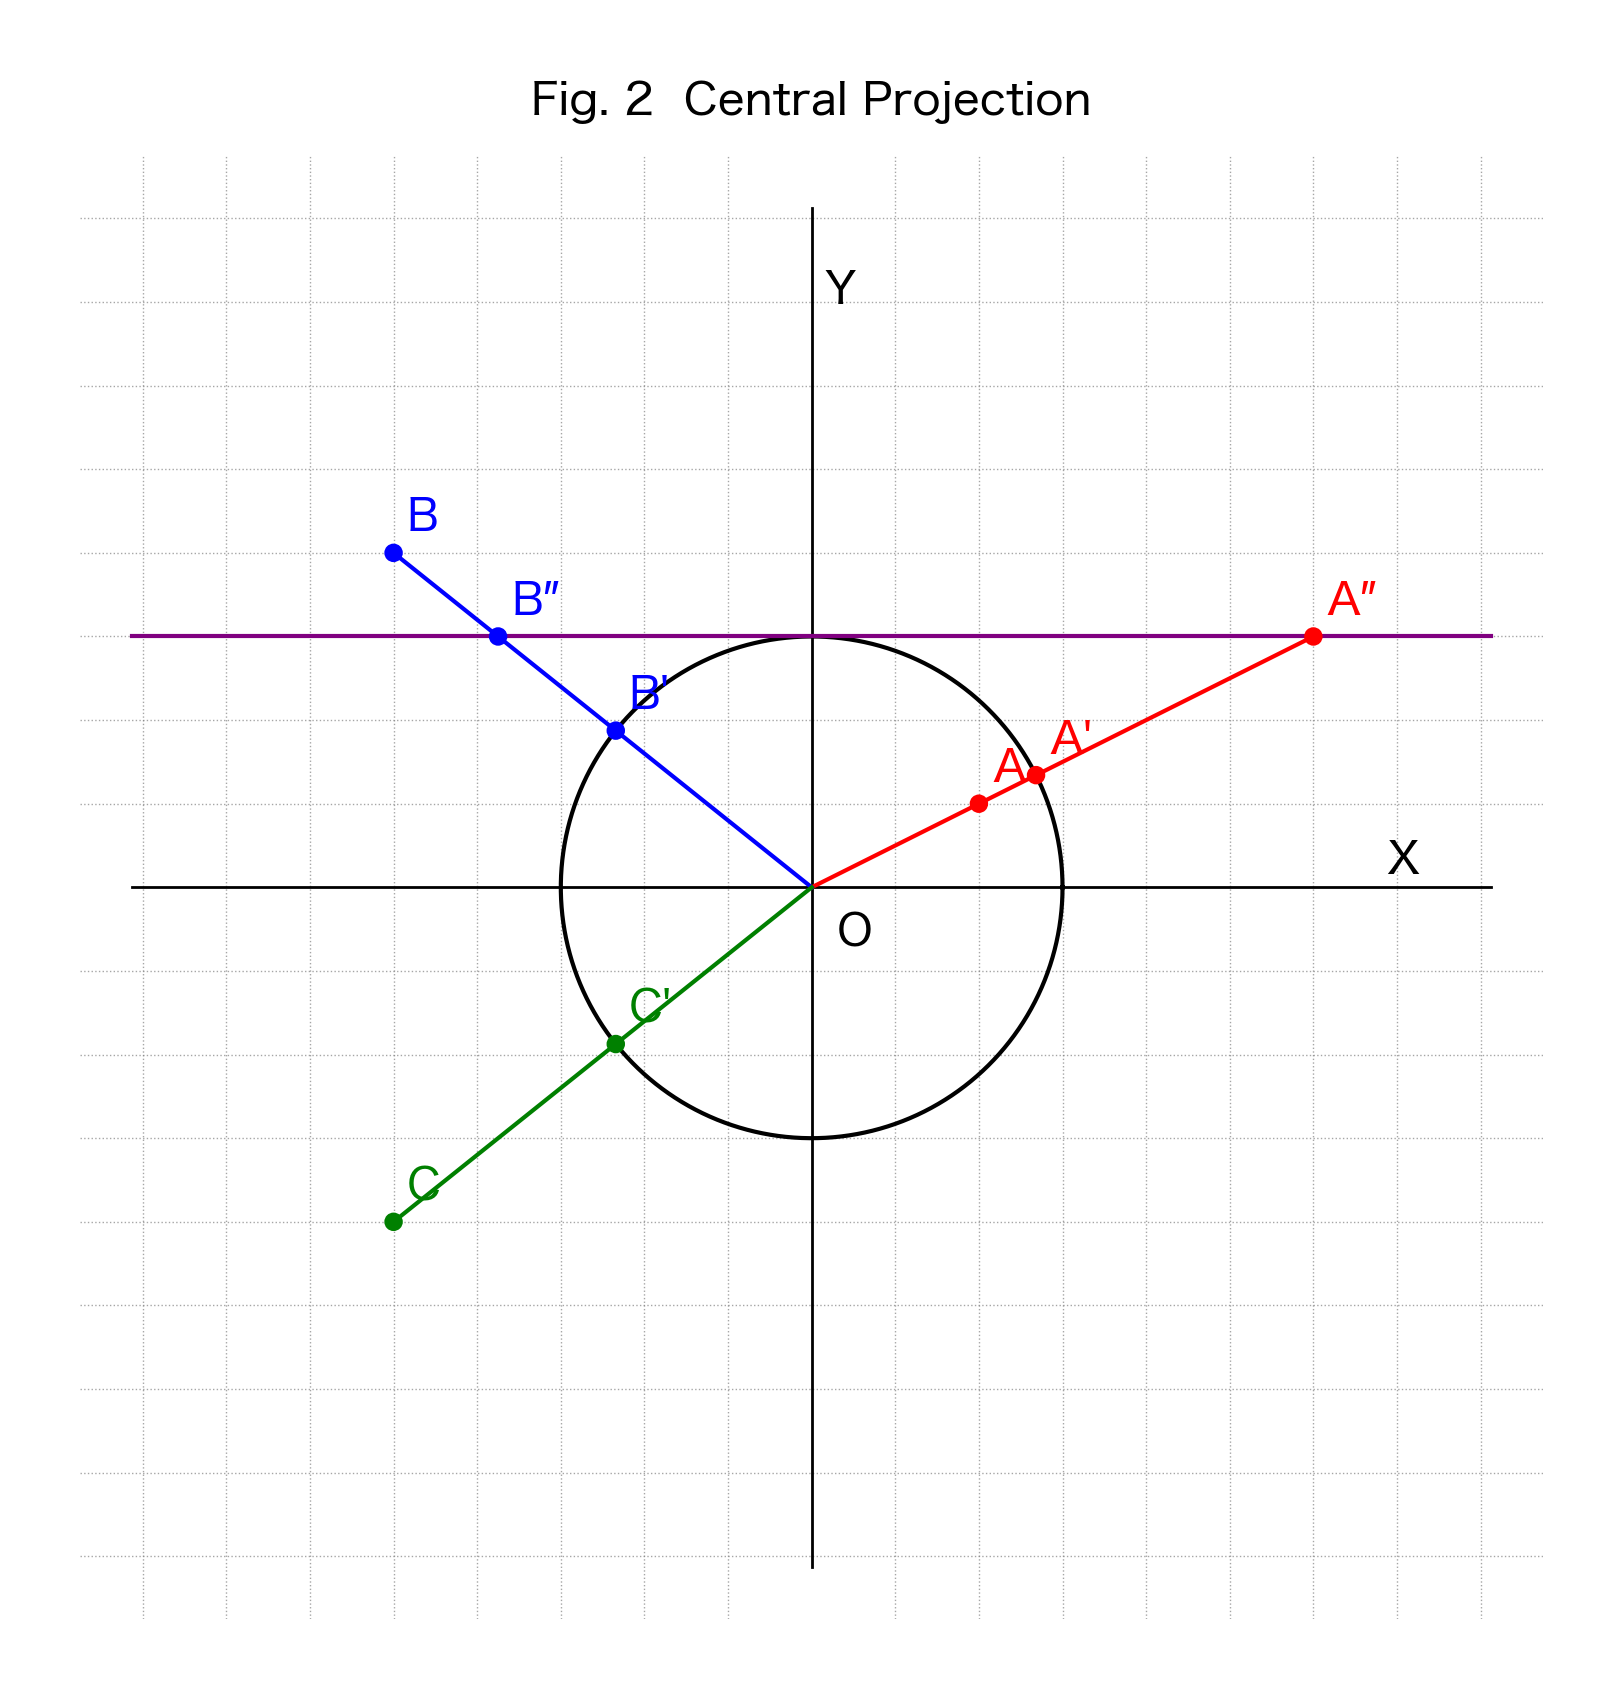
\includegraphics[keepaspectratio,alt={Fig. 2 Central Projection}]{fig2_central_projection.png}}
\caption{Fig. 2 Central Projection}
\end{figure}

\textbf{図 2}：中心投影 \(\Phi_R\)
の図解（\(n=1\)、\(R=3\)）。北極で接する接超平面（紫線、\(n=1\) のとき
\(y = R\)、一般には式 (3.1) の \(x_{n+1} = R\)）上の点 \(A'', B''\)
を、原点 \(O\) を視点とする放射状半直線で球面上の \(A', B'\)
に投影する。同じ放射線で球面投影 \(\sigma_R\)
も定義されており、両者の唯一の違いは定義域である。\(\Phi_R\)
の像は開上半球（南半球には到達せず、赤道にも有限点からは到達しない）。緑の
\(C, C'\) は球面投影 \(\sigma_R\) の例であり、中心投影 \(\Phi_R\)
の像（開上半球）には含まれない。

\subsection{3.5
既存結果との関係}\label{ux65e2ux5b58ux7d50ux679cux3068ux306eux95a2ux4fc2}

\textbf{注釈 3.1（既存結果の書き換え）}：{[}1{]} および {[}2{]} において
\(\Phi_R\) により定義された幾何量（誘導計量
\(g_{\mu\nu} = \Phi_R^* g_{S^n(R)}\)、Einstein テンソル、合成曲率半径
\(r_{\text{final}}^2 = r_1^2 - \sum_{j \in S}(x_{i_j}^*)^2\)
等）は、本ノートの記法では \(\sigma_R \big|_{\Pi_R}\)
による引き戻しとして書き換え可能。

ただし、これらの幾何量は本質的に
\(\Pi_R\)（上半球面）上の構造であり、球面投影 \(\sigma_R\)
の定義域拡張への自動的な拡張は意味しない。一般の滑らかな写像
\(f: M \to N\) の引き戻し \(f^* T\) は写像の単射性によらず well-defined
であり、特に \(\sigma_R^* g_{S^n(R)}\) は
\(\mathbb{R}^{n+1} \setminus \{0\}\) 上の well-defined な対称 2
テンソルである。しかし命題 2.4 により動径方向 \(\mathrm{span}\{x\}\)
が微分の核に入るため、この引き戻しテンソルは退化しており、リーマン計量ではない。したがって、\(\Phi_R^* g_{S^n(R)}\)
が \(\Pi_R\) 上に与える非退化な誘導計量と同一視することはできない。

{[}2{]} の切断操作（本ノートでは記号衝突回避のため \(\kappa_S\)
と書く）の半群構造、可換性、合成曲率半径の閉形式は、\(\sigma_R\)
の像空間 \(S^n(R)\) 上の操作として位置付けられる。

\begin{center}\rule{0.5\linewidth}{0.5pt}\end{center}

\section{§4 結語}\label{ux7d50ux8a9e}

\subsection{4.1
本ノートの主要結果}\label{ux672cux30ceux30fcux30c8ux306eux4e3bux8981ux7d50ux679c}

\begin{enumerate}
\def\labelenumi{\arabic{enumi}.}
\tightlist
\item
  球面投影 \(\sigma_R(x) = (R/\|x\|) x\) を
  \(\mathbb{R}^{n+1} \setminus \{0\}\) から \(S^n(R)\) への \(C^\infty\)
  級レトラクションとして明示的に定義した（定義 2.1、命題 2.1）。
\item
  冪等性、変形レトラクト構造、商空間表示、微分の核と像、角度保存、スケール不変性を初等的に整理した（命題
  2.2 〜 2.6）。
\item
  中心投影 \(\Phi_R\) は球面投影 \(\sigma_R\) を接超平面 \(\Pi_R\)
  に制限したものに等しく、その像は\textbf{開上半球面 \(S^n_+(R)\)}
  であり、\(\Phi_R\) は微分同相である（定義 3.1、命題 3.1、補題 3.2）。
\item
  \(\sigma_R\) の非単射性と \(\Phi_R\) の単射性の対比を §3.4
  に整理した。
\end{enumerate}

\subsection{4.2 位置付け}\label{ux4f4dux7f6eux4ed8ux3051}

本ノートで定義された球面投影 \(\sigma_R\) は、位相幾何学において
\textbf{radial projection}
として古典的に既知の写像と同一である（{[}Hatcher Ch.0{]}
等）。本ノートの貢献は新規の幾何学的定理の発見ではなく、

\begin{itemize}
\tightlist
\item
  この基礎写像を「球面投影
  \(\sigma_R\)」として明示的に命名・記号固定すること
\item
  著者の中心投影フレームワーク {[}1{]}, {[}2{]}
  における操作との関係を明示的に整理すること
\end{itemize}

に限定される。本ノートは中心投影シリーズの基礎を固めるための
\textbf{Zenodo
プレプリント／テクニカルノート}として公開し、純粋数学ジャーナル投稿は意図しない。

\subsection{4.3
本ノートが主張しないこと}\label{ux672cux30ceux30fcux30c8ux304cux4e3bux5f35ux3057ux306aux3044ux3053ux3068}

\begin{itemize}
\tightlist
\item
  球面投影 \(\sigma_R\)
  が「先行研究において発見されていなかった」こと（radial projection
  として古典的に既知）。
\item
  球面投影 \(\sigma_R\)
  に関する深い数学的結果（部分多様体論、極作用、等径関数、共形性等との一般的対応）。
\item
  球面投影 \(\sigma_R\) が中心投影 \(\Phi_R\)
  の単なる定義域拡張により、\(\Phi_R\)
  の豊かな幾何構造（誘導計量・曲率テンソル等）が自動的に \(\sigma_R\)
  に継承されること（実際は単射性が失われるため、引き戻しは制限 \(\Pi_R\)
  上でのみ well-defined）。
\item
  物理的応用、宇宙論的解釈、量子論的含意等。
\end{itemize}

これらは別ノートまたは別論文において扱う。

\begin{center}\rule{0.5\linewidth}{0.5pt}\end{center}

\section{参考文献}\label{ux53c2ux8003ux6587ux732e}

{[}1{]} Kihara, N. (2026).
\emph{中心投影による4次元空間の幾何学的定式化}. Zenodo. Concept DOI:
\href{https://doi.org/10.5281/zenodo.19427780}{10.5281/zenodo.19427780}.

{[}2{]} Kihara, N. (2026).
\emph{中心投影の合成演算と合成曲率半径の閉形式：1
回の中心投影と球面上の可換切断による高次元削減の代数的定式化}. Zenodo.
Concept DOI:
\href{https://doi.org/10.5281/zenodo.20060728}{10.5281/zenodo.20060728}.

{[}3{]} A. Hatcher (2002). \emph{Algebraic Topology}. Cambridge
University Press. （Chapter 0: deformation retract \(r(x) = x/\|x\|\)）

\begin{center}\rule{0.5\linewidth}{0.5pt}\end{center}

著者：木原 範昭（Noriaki Kihara） 所属：WF System Co., Ltd.
ORCID：\href{https://orcid.org/0009-0004-6753-4020}{0009-0004-6753-4020}
ライセンス：CC BY 4.0

\begin{center}\rule{0.5\linewidth}{0.5pt}\end{center}

\subsection{改訂履歴}\label{ux6539ux8a02ux5c65ux6b74}

\begin{itemize}
\tightlist
\item
  \textbf{v1（2026-05-30 第一稿）}：初版。
\item
  \textbf{v2（2026-05-30 改訂）}：4 AI
  査読（Claude.ai、ChatGPT、Gemini、Grok）の指摘を統合反映：

  \begin{itemize}
  \tightlist
  \item
    命名：「球面投影」を保持しつつ「radial projection と同一」を §1
    で明示
  \item
    位置付け：テクニカルノート/Zenodo プレプリントとして明記
  \item
    中心投影の像を開上半球面 \(S^n_+(R)\) と明示（命題 3.1）
  \item
    「角度保存性」を真の角度保存（命題
    2.5、内積式）に厳密化、別途スケール不変性（命題 2.6）に分離
  \item
    追加命題：冪等性（命題 2.2）、商空間（命題 2.3）、微分の核（命題
    2.4）
  \item
    「上位概念」「標準テキスト存在せず」の主張を弱化
  \item
    系 3.1(ii) を注釈 3.1 に格下げ、自己完結化
  \item
    外部文献 Hatcher を追加（参考文献 {[}3{]}）
  \item
    記号 \(\sigma_S\) → \(\kappa_S\) に変更（{[}2{]} 切断操作）
  \item
    「位相」→「方向成分」全文置換
  \item
    \(t<0\) の扱いを脚注で補足
  \item
    中心投影 \(\Phi_R\) と古典 gnomonic projection の向きの差異を
    §1.2、§3.1 で明示
  \item
    Well-definedness を定義直後に明記
  \end{itemize}
\item
  \textbf{v3（2026-05-30 微修正）}：ChatGPT v2 再査読の指摘を反映：

  \begin{itemize}
  \tightlist
  \item
    命題 2.4 の核の証明を正しく書き直し（\(D\sigma_R|_x(v)=0\) から
    \(v=\lambda x\) の同値性を示す形式に）
  \item
    §3.5 注釈 3.1 の「引き戻しは well-defined でない」を「well-defined
    だが退化する」に修正（引き戻しは単射性に依らず常に
    well-defined、問題は退化）
  \item
    Fig. 3 キャプションを命題 2.6 のみ参照に修正（命題 2.5 削除）
  \item
    Fig. 2 キャプションに緑 \(C, C'\) が中心投影像に含まれない旨を補足
  \item
    §1.1 「primary な named operation
    として独立文書は存在しない」を「シリーズ内での参照基盤として有用」に弱化
  \item
    Fig. 2 キャプションに「\(n=1\) のとき \(y = R\)、一般には式 (3.1) の
    \(x_{n+1} = R\)」を補足（Gemini v2 再査読指摘）
  \end{itemize}
\item
  \textbf{v3.1（2026-05-30 微修正）}：Claude.ai v2
  再査読の軽微指摘を反映：

  \begin{itemize}
  \tightlist
  \item
    命題 2.4 に微分の像
    \(\mathrm{Im}(D\sigma_R|_x) = x^\perp = T_{\sigma_R(x)} S^n(R)\)
    を追記（式 2.4）。沈め込み構造をより明示的にし、\(\sigma_R(x)\)
    における球面の接空間が動径方向の直交補空間と一致することを明記。
  \end{itemize}
\item
  \textbf{v3.2（2026-06-02 校正・推敲）}：査読指摘の校正・推敲を反映：

  \begin{itemize}
  \tightlist
  \item
    式番号の重複を解消：命題 2.5（角度保存）の式を (2.4) から
    \textbf{(2.5)} に振り直し（命題 2.4 の像の式 (2.4)
    と衝突していた）。
  \item
    §1.2 の相互参照を「補題 3.1」から正しい「\textbf{補題 3.2}」に修正。
  \item
    命題 2.4 の証明に\textbf{像 \(\mathrm{Im} = x^\perp\)
    の論証}（\(x \cdot D\sigma_R|_x(v) = 0\)
    と階数・退化次数定理）を追記。従来は核のみで像の根拠が欠けていた。
  \item
    命題 2.4
    の見出しを「微分の核」から「\textbf{微分の核と像}」に変更（内容に整合）。§4.1
    第2項も同様に更新。
  \item
    §3.4 表の \(\Phi_R\)
    動径方向の欄を「定義域に動径方向ない」から「\textbf{核の方向が定義域の接空間に含まれない（横断的）}」に厳密化。
  \item
    命題 2.4 証明冒頭の微分を、曖昧な \(\frac{d}{dx}\)
    表記から「\textbf{方向 \(v\) に沿った微分}」へ明確化。
  \end{itemize}
\end{itemize}

\end{document}
